% Two maps of Congress: the paper at six pages. Rebuilt 25 Nov 2026 by Martin with Claude from the version the group
% printed and commented on (v2: report/main.tex and report/sections/*.tex; comments in ../v2_comments_SGAI_PAPER.pdf).
% v2's wording, subsections and run-in headings are kept wherever no comment asked for a change; each change is named
% in a % line. Figure 4 and its paragraph come from the full draft (Anas, 25 Nov). DECISIONS G22 and G23.
% Nothing here is a new analysis except the delegation check (Martin/delegation_check/, G23).
\documentclass[9pt,twocolumn,twoside]{pnas-new}
\articletype{Political Sciences}
\templatetype{pnasresearcharticle}

% Less whitespace around figures: tighter gaps between floats and text, a shorter gap to the caption, and
% float fractions that let text fill the rest of a column instead of leaving a float alone on a page.
\setlength{\textfloatsep}{8pt plus 2pt minus 2pt}
\setlength{\dbltextfloatsep}{8pt plus 2pt minus 2pt}
\setlength{\floatsep}{6pt plus 2pt minus 2pt}
\setlength{\dblfloatsep}{6pt plus 2pt minus 2pt}
\setlength{\intextsep}{6pt plus 2pt minus 2pt}
\captionsetup[figure]{skip=4pt}
\renewcommand{\topfraction}{0.95}
\renewcommand{\dbltopfraction}{0.95}
\renewcommand{\textfraction}{0.05}
\renewcommand{\floatpagefraction}{0.9}
\renewcommand{\dblfloatpagefraction}{0.9}

\begin{document}

\title{Two maps of Congress: the House is less divided in whom its members name than in whom they work with}

\author[a]{Anas Mir}
\author[a]{Martin M{\o}llenhus}
\author[a]{Diego A. Mijares}
\affil[a]{Technical University of Denmark, 02805 Social Graphs and Interactions}

\leadauthor{Mir}

% Martin's 26 Nov comment: rewritten to open on the finding (also fills more of page 1's right column).
\significancestatement{The US House looks less divided when you ask whom its members name than when you ask whom they
work with. Polarization is usually measured from votes or vocabulary, and both show two camps. We drew the same 450
members twice. On the floor, members name colleagues of the other party more often than they cosponsor bills with
them, and mostly to give them credit. In press releases, members in close districts name the other party most, and
mostly name partners. How polarized Congress looks depends on the record you choose, and a named partner, unlike the
word ``bipartisan'', can be checked against the bills.}

% Comment 2: written from the owners in WORK_AND_DEADLINES.md section 2, so each line credits what that author did.
\authorcontributions{M.M. built the shared name matcher, the floor and working maps, their null models and community
analysis, the null for cited bills and the delegation check, made Figure 1, and wrote the Results and Methods on the
two maps. A.M. built the press-release collector, collected the 55,023 releases and matched them to members and
bills, measured district lean, ran the close-up analysis and its checks, the home map and the analysis of
``bipartisan'' releases, made Figures 3 and 4, and wrote the Results and Methods on the close-up. D.A.M. wrote the
labelling rules, coded the 100 labelled mentions, measured the matcher's precision and the speaker attribution, built
the text classifier, compiled the literature and the record of AI use, made Figure 2, and wrote the Results and
Methods on what mentions mean. M.M. and A.M. second-coded the labelled mentions; D.A.M. and M.M. wrote the
Introduction and Discussion; all authors read and revised the paper. Code and text were first drafted with an AI
assistant (Claude, Anthropic) and then rewritten and extended by the authors (Methods, AI use).}
\authordeclaration{The authors declare no competing interest.}
\correspondingauthor{}

\keywords{Congress $|$ polarization $|$ networks $|$ floor speech $|$ press releases}

% Comment 1: v2's abstract, with the press releases given room in proportion to part 3. 150 words (course).
\begin{abstract}
House members vote along party lines, but how divided are they in whom they name? We draw the
119th House (2025--2026) twice on the same 450 members: a working map, where two members are joined when one
cosponsors the other's bill, and a floor map, where they are joined when one names the other in a floor speech. At
equal size, 38.7\% of floor ties cross the party line against 28.6\% of working ties, and debate procedure explains
about two thirds of the floor map's division. Hand-coding 100 mentions shows that cross-party mentions are mostly
thanks and credit (69\%) and rarely disagreement (7\%). In 55,023 press releases, members in exposed seats name the
other party more often than safe-seat members, and mostly name partners, though seat and moderation cannot be
separated. The same members look more or less divided depending on the record read: bills, floor speeches or
press releases.
\end{abstract}

\dates{Hand-in 27 November 2026.}

\maketitle
\thispagestyle{firststyle}
\ifthenelse{\boolean{shortarticle}}{\ifthenelse{\boolean{singlecolumn}}{\abscontentformatted}{\abscontent}}{}

% Page 1: text in one wider block, Significance box on the right (template). Page 1 ends at the \Parasplit below.
% When text before it changes, move \Parasplit to the last word on page 1.
\Firstpage

% ================================================================ INTRODUCTION
% v2's introduction (Diego and Martin). Comment 3: the literature in paragraphs 2 and 3 is given as what each study
% found. Roll-call votes are defined at first use, exposed seats in the last paragraph (Q6).

\dropcap{T}he United States Congress is usually described as two camps, and most ways of measuring it agree.
Members of the two parties vote apart, and they have used increasingly different words since the early 1990s
\cite{gentzkow2019}. Networks built from who signs whose bills show the same split, with ties between the parties
growing rarer and more hostile over four decades \cite{neal2020}.

How deep the split looks depends, however, on which record is read. Harbridge finds that between 1973 and 2004,
bipartisan agreement fell in roll-call votes, the recorded votes in which each member's yes or no is published, while
staying far more stable in cosponsorship, and traces this to party leaders choosing which bills reached a vote
\cite{harbridge2015}. Across communication channels, Green and colleagues find the parties always distinguishable,
but more so in front of national audiences than local ones \cite{green2024}. Division, on this evidence, is a
property of the measurement as well as of the institution.

Members also have reasons to manage how divided they appear. In survey experiments, voters with weak party
attachments rewarded a bipartisan image \cite{harbridge2011}, and Grimmer reads what members say to constituents as a
strategic presentation of their work \cite{grimmer2013}. That presentation need not match the work: Westwood finds
that floor speeches calling a bill bipartisan mostly concern bills with trivial support from the other party, and
that a member's bipartisan rhetoric is unrelated to their bipartisan votes \cite{westwood2022}.

We compare two records of the same 450 members of the House in the 119th Congress (2025 to 2026). The first, the \emph{working map}, is the cosponsorship network \cite{fowler2006}: two members are tied when one
signs a bill the other sponsors. The second, the \emph{floor map}, is to our knowledge new: two members are tied when
one names the other in a floor speech. Both are networks on
identical nodes, so the same measures of party division apply to each and both can be tested against the same
null models. A word such as ``bipartisan'' costs nothing to say. A name points at a specific colleague, and what is
said about that colleague can be read.

Whether naming is more or less partisan than working cannot be guessed in advance. Members might attack the other
side in public and cooperate quietly, or display the few cross-party partners they have. We find that members name colleagues of the other party more readily than they cosponsor with them, that debate procedure accounts for much, but not all, of the\Parasplit
floor map's own party division, and that cross-party mentions are mostly acknowledgement rather than
argument. At home, in press releases, members
in exposed seats, whose district leans toward their own party by five points or less, name the other party more often
than members in safe seats, and mostly name partners.

% ================================================================ RESULTS
% Draft 27 Nov (Martin with Claude): Results rewritten in the style of Sekara et al. (PNAS 2016): short run-in
% headings, each paragraph says what was asked and what was found with its one or two key numbers; ranges, sample
% sizes, secondary p-values and check-by-check detail moved to the figure captions and Methods. No number changed.
\section*{Results}

\subsection*{Two maps of the same House}

% Martin's 26 Nov comment: more width to the figure, a narrower and longer caption, less blank space above it.
\begin{SCfigure*}[0.4][t]
\centering
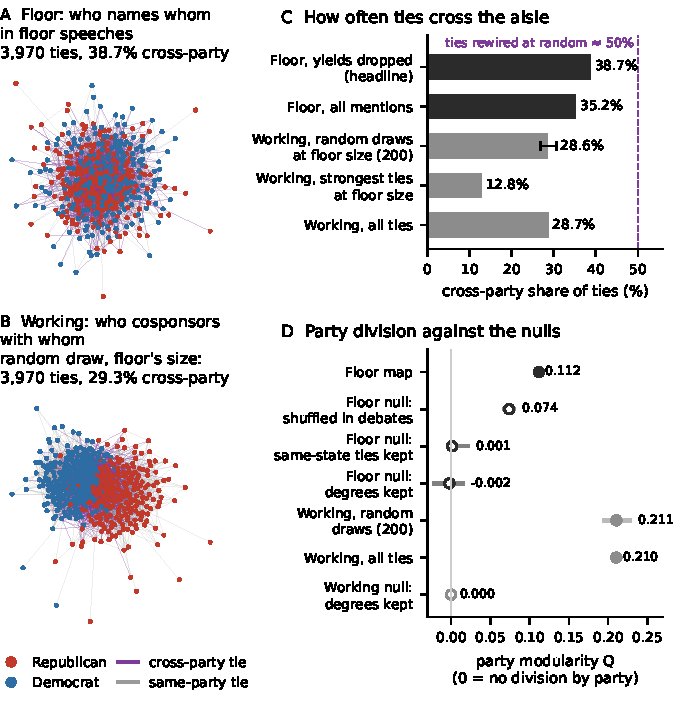
\includegraphics[width=12.4cm]{figures/figure1_side.pdf}
\caption{The House as two networks, January 2025 to November 2026. (\emph{A}) Floor map: members tied when one names
the other in a floor speech, yields (handing over debate time) left out. (\emph{B}) Working map: one random draw of
sponsor--cosponsor ties, thinned to the floor map's 3,970 ties. Nodes are members (red Republican, blue Democrat);
purple ties cross the aisle. Positions come from a spring layout and carry no meaning. (\emph{C}) Share of ties that
cross the aisle; the bar for the random draws shows the range over 200 draws, and the dashed line the level expected
if ties were rewired at random. (\emph{D}) Party modularity of each map (filled) against its nulls (open; lines show
the range over the draws). At every comparison a larger share of floor ties than of working ties crosses the aisle, and the floor map is still more
divided than every null.}
\label{fig:maps}
\end{SCfigure*}

We built two networks on the same 450 Republicans and Democrats of the 119th House. In the \emph{working map}, built from cosponsorship, two members are tied when one cosponsored a bill that the other sponsored. In the \emph{floor map}, they are tied when
one named the other in a floor speech. We leave out yields, the moments when the member managing a debate hands
speaking time to a colleague by name (``I yield 2 minutes to the gentleman from Texas''), because they are procedure
rather than a choice to name someone (Methods).

\textbf{More naming than cosponsoring.} On the floor, 38.7\% of ties join a Republican and a Democrat
(Fig.~\ref{fig:maps}\emph{A} and \emph{C}). The working map is twelve times denser, so we compare like with like by
drawing working ties at random until both maps have the same size. Then 28.6\% of working ties cross the aisle, and
none of 200 draws comes close to the floor map (Fig.~\ref{fig:maps}\emph{B} and \emph{C}). Party modularity tells the
same story, 0.112 on the floor against 0.211 for the draws (Fig.~\ref{fig:maps}\emph{D}), and the gap does not depend
on leaving out yields (Methods). Members' closest working partnerships are the most partisan of all: among the pairs
who share the most bills, only 12.8\% cross the aisle.

\textbf{Chance and debates.} Both maps are far more divided than chance: if ties were rewired at random, about half
would cross the aisle (Fig.~\ref{fig:maps}\emph{C}). Part of the floor map's division, though, comes from how
debates are run. Each debate has its own cast of speakers, often with a manager from each party. When we shuffle who
is named only within each debate, modularity falls from 0.112 to 0.074, so the debates account for about two thirds
of the division. The last third, members naming their own side more than the debate requires, is larger than in any
of 200 shuffles. State delegations explain almost none of it (Methods).

\textbf{Committees.} The two maps also fall into different communities. Louvain splits the working map into the
two parties (normalised mutual information with party, NMI, 0.83). On the floor map it finds eight communities that
each hold both parties (NMI 0.03). Seven of them gather around one committee, such as Appropriations or Ways and
Means, and the eighth holds the party leaders. Almost half of floor ties (44\%) join two members of the same
committee, against 17\% if ties were placed at random (Methods). Crossing the aisle on the floor is largely
committee work, and the next section reads what these mentions say.

\subsection*{What a cross-party mention means}

Naming a colleague is not working with them, and a member can name the other side to attack it. To see what the
cross-party ties are, we read 100 floor mentions drawn at random and coded what the speaker was doing towards the
named member (Methods). Most cross-party mentions give credit: 69\% thank a bill's co-lead or a committee's chair,
praise joint work or support the member's bill. Another 23\% are neutral, such as naming the member who introduced
a bill. Only 7\% disagree with the named member (Fig.~\ref{fig:labels}), and handing over debate time never crosses
the aisle.

We tried to carry these labels to all 9,909 floor mentions with a text classifier, but it did no better than always
guessing ``agreeing'' (Methods), so we report the hand-coded shares only. On the floor, members name the other side
to credit it far more often than to oppose it.

\begin{figure}[t]
\centering
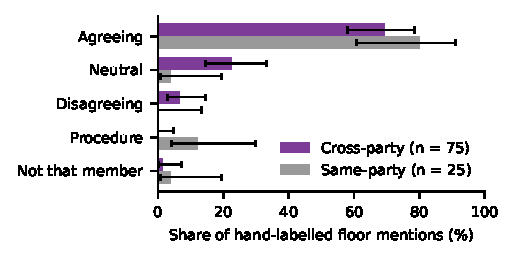
\includegraphics[width=8.7cm]{figures/figure2.pdf}
\caption{What floor mentions do. Share of 100 hand-labelled mentions in each code, for mentions between parties
(purple, $n = 75$) and within a party (grey, $n = 25$). Lines show 95\% Wilson intervals. Codes as in Methods; a
mention was coded ``not that member'' when the matcher gave the name to the wrong person (for example the wrong
Wilson, or a constituent). Cross-party mentions are mostly
agreeing and rarely disagreeing; procedure appears only within a party.}
\label{fig:labels}
\end{figure}

\subsection*{Close-up: whom members name at home}

\begin{figure}[!t]
\centering
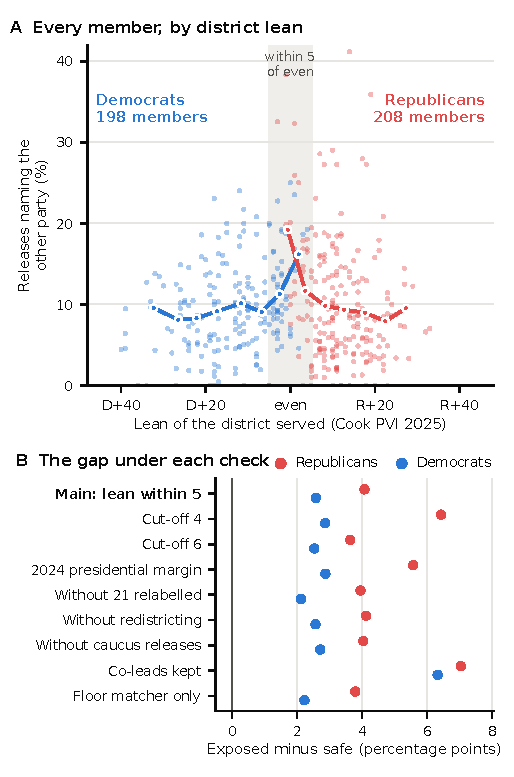
\includegraphics[width=8.7cm]{figures/figure3.pdf}
\caption{\textbf{Members in exposed seats name the other party more often in their press releases.} (\emph{A}) Each
dot is one of 406 House members (198 Democrats, 208 Republicans; 53,664 releases, 3 January 2025 to 20 November
2026): the share of their releases that name a House member of the other party who is neither a party leader nor a
co-lead of a bill the release cites, against the lean of the district they served (Cook PVI 2025). Lines join the
mean share in 5-point bands of lean (bands with at least five members). Shading marks districts within five points of
even. (\emph{B}) Exposed minus safe mean share, by party, for the main definition (top) and for each check fixed
before the analysis (Methods). Every gap is positive with $p < 0.05$ (labels shuffled within party, 10,000
shuffles).}
\label{fig:home}
\end{figure}

We asked whether members whose seat is at risk name the other party more in their own press releases. For the 406
members with at least ten releases, we measured how often a release names a House member of the other party who is
neither a party leader nor a co-lead of a bill the release cites. A seat is exposed when the district leans toward
the member's own party by five points or less (Cook PVI 2025 \cite{cook2025pvi}). In both parties, exposed members
name the other side more: 13.3\% of releases against 9.2\% for safe Republicans, and 11.6\% against 9.0\% for
Democrats ($p = 0.004$ for each; Fig.~\ref{fig:home}).

\textbf{Closest seats.} The difference comes from the closest seats. The closest of the exposed seats, where the district is even or leans to the other party (8 of the 37 exposed
Republicans and 10 of the 54 exposed Democrats), name it most, in about one release in five for Republicans; beyond five points of lean the share is
nearly flat (Fig.~\ref{fig:home}\emph{A}). The gap survives every check we fixed before the analysis
(Fig.~\ref{fig:home}\emph{B}). It also does not come from members simply having more colleagues of the other party
in their home state's delegation (Methods).

\textbf{Partners.} A count says nothing about tone. Three AI readers (Claude models from Anthropic; Methods), who did
not see the seat, read 60 of the counted names: 46 named a partner or praised the member, and only one criticised.
At home, as on the floor, cross-party names are mostly acknowledgement.

\textbf{Moderates.} Exposed members are also their party's moderates, and our data cannot separate the two. We
measure ideology with DW-NOMINATE, a standard score that places each member from liberal to conservative by their
roll-call votes; a moderate is a member whose votes place them close to the other party. About half of the exposed
members are in their party's most moderate fifth. Comparing exposed and safe members of similar ideology leaves
little of the gap: 1.1 of 4.1 points for Republicans and 0.2 of 2.6 for Democrats (Methods). This check may ask too
much, though. An exposed seat may itself push a member to vote more moderately, and then holding ideology fixed also
removes part of the seat's own effect.

\begin{figure*}[!t]
\centering
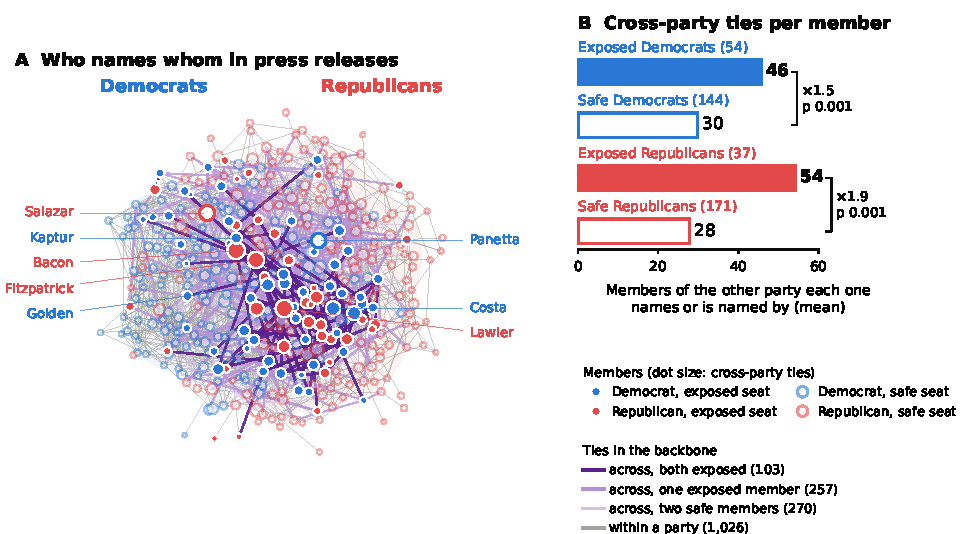
\includegraphics[width=17.8cm]{figures/figure4.pdf}
\caption{Who names whom in press releases. (\emph{A}) Each dot is one member ($n = 406$), placed by ForceAtlas2 on the
backbone of naming ties (disparity filter, $\alpha = 0.01$). Filled dots: exposed seats; hollow dots: safe seats; dot
size: number of cross-party ties. Purple lines cross the aisle, darkest between two exposed members; grey lines stay
within a party. Positions illustrate the network and are not a measurement. (\emph{B}) Members of the other party each
member names or is named by, on average: exposed members have 1.5 (Democrats) and 1.9 (Republicans) times as many as
safe members ($p = 0.001$, exposure shuffled within party, Holm-corrected over ten comparisons). Exposed members of
both parties sit where the two parties meet.}
\label{fig:homemap}
\end{figure*}

\textbf{The home map.} Tying two members when one names the other gives a home map of the same 406 members
(Fig.~\ref{fig:homemap}). Exposed members are its hubs. They are 22\% of members but take part in about a third of
its cross-party ties, and they are tied to more members of the other party than safe members are, 1.9 times as many
for Republicans and 1.5 times for Democrats (Fig.~\ref{fig:homemap}\emph{B}). On the backbone, which keeps each
member's strongest ties \cite{serrano2009}, the parties differ. Exposed Republicans bridge by volume, with more
backbone ties than safe Republicans. Exposed Democrats bridge by position: they have as many ties, but sit on more of
the shortest paths between members than those ties predict (Methods). We did not test why. One possibility is that
the majority's control of the floor agenda gives exposed Republicans more occasions to name Democrats.

\textbf{``Bipartisan''.} A quarter of the releases call something bipartisan, and most of them back the word with a
partner: 64\% name a House member of the other party or cite a bill one co-leads, against 9\% of other releases.
Three AI readers confirmed that the members named are partners, not opponents (Methods). Here the parties swap roles.
Exposed Democrats back the word with a partner more often than safe Democrats (63.0\% against 56.7\%, $p = 0.012$),
while Republicans in exposed and safe seats do not differ.

\textbf{Cited bills.} Members also cite their cross-party bills more often than their other bills: 52.7\% of the
bills they sponsored with an original cosponsor from the other party appear in their press releases, against 45.1\%
of the rest ($p < 0.001$). Most of that gap, however, separates co-led bills from solo bills. Against bills co-led
only by the member's own party, the gap shrinks to 3.5 points ($p = 0.02$). Bipartisan bills may also be cited more
because they pass more often, which our data cannot test.

% ================================================================ DISCUSSION
% v2's discussion (Diego and Martin). Comment 7: the last paragraph says what we were limited by, defines exposed seats
% and roll-call votes again in a few words, and draws no conclusion the data cannot carry.
\section*{Discussion}

Drawn from the same members over the same two years, the House looks less divided in whom its members name on the
floor than in whom they work with. The difference holds when both maps have the same number of ties, when yields
of debate time are left out, and against a null model that keeps who took part in each debate. Hand-labelled
mentions say what the cross-party ties are: mostly thanks and credit, rarely argument. The floor is where
cross-party work is acknowledged, typically by the managers of a bill and the leaders of its committee.

The result does not show that members cooperate more than cosponsorship suggests. A mention is a reference, made
in a setting where House procedure brings members of both parties into the same debates; that procedure accounts
for about two thirds of the floor map's party division, and the communities of the floor map follow committees,
not parties. Part of what we measure is therefore the committee system at work in public. The comparison also
depends on how the dense working map is thinned: against random ties of the same number the gap is ten points,
against members' strongest partnerships (12.8\% cross-party) it is much wider.

Several limits are our own findings. The name matcher was right in 98 of 100 hand-labelled mentions and found 12
of 13 names in 30 turns read in full, so recall rests on few names. Wrong matches are not neutral: a constituent or a
namesake mistaken for a member belongs to the other party about half the time, and on an earlier version of the
matcher five of seven errors joined members of different parties. Errors of this kind push the floor map towards
looking less divided; at 98\% precision the effect on the headline is small, but it runs in the direction of our
finding. One hundred labels give wide intervals and too few disagreements for a text classifier to learn from: ours
did not beat always answering ``agreeing''. Party was hidden on the coding sheets, but coders often know a member's
party, so the coding was not blind in practice. The AI readers in the press-release checks are one model family, so
their agreement shows that they are stable, not that they are right; a person read every case where they disagreed.

Where Westwood found that the word ``bipartisan'' is detached from votes \cite{westwood2022}, the names members use
across the aisle on the floor are mostly credit for specific bills and committee work, and at home the word mostly
comes with a named partner. In their press releases, members in exposed seats, whose district leans toward their own
party by five points or less, name the other party more often than members in safe seats, in both parties, and
mostly name partners. Why, our data cannot say. Exposed members are also their party's moderates, and among members of
similar ideology little of the gap remains (1.1 of 4.1 points for Republicans, 0.2 of 2.6 for Democrats). Ideology
is measured from roll-call votes, the published yes or no of each member, and an exposed seat may itself make a member
vote more moderately, so the seat and the ideology cannot be separated with these data. In this House the president's
party is also the majority, so a president's-party effect cannot be told from a majority effect either. We were also limited to one Congress and one
chamber, which cannot say whether these patterns are stable, and to press releases, which miss newsletters and social
media. We did not test, pair by pair, whether each named colleague is also a cosponsorship partner; that is the
natural next check. The same two maps can be drawn for any Congress since the Record went online.

% ================================================================ METHODS
% v2's methods (Martin: from_martin_methods.tex; Diego: methods.tex; Anas: methods_press.tex). Comment 8: shortened
% to each source with its counts, each choice that changes a number and each validation with its result; the AI-use
% paragraph is expanded. Step-by-step detail stays in the repository.
\matmethods{
\subsection*{Data}
Members are the 450 Republicans and Democrats who served in the 119th House, identified by Bioguide ID (Voteview
\cite{voteview2026}, with unitedstates/congress-legislators for names). Floor speech comes from the Congressional
Record on govinfo.gov, 6 January 2025 to 9 November 2026, split into speaker turns; we keep the 17,824 House-floor
turns of at least 50 words spoken by a member. Bills and cosponsorships come from govinfo's BILLSTATUS bulk data for
the same Congress. All 60 turns checked by hand were assigned to the member the Record names as speaker (95\% Wilson
interval \cite{wilson1927}, 94\% to 100\%).

\subsection*{Finding names}
A rule-based matcher finds each member named in a turn: a House title followed by a surname (``Mr. Cole'', ``Speaker
Johnson''), names in lists after a plural title (``Representatives Lawler, Golden, and Fitzpatrick''), and full names
without a title (``my friend, Chip Roy''). Shared surnames are settled by first name or nickname and then by a state
name within 80 characters; otherwise the name is dropped. Names after ``Senator'', ``Governor'' and similar titles are
skipped, and a member naming themselves is not counted. On 100 hand-labelled mentions, 98 named the right member
(lists and untitled names, added later, were checked separately: 20 of 20 and 30 of 30 right); in 30 randomly drawn
turns, the matcher found 12 of the 13 members a reader found (recall, 92\%).

\subsection*{Yields}
When a floor manager hands debate time to a member (``I yield 2 minutes to the gentleman from Texas''), the name is
procedure, not a choice to name someone. We flag a mention as a yield when ``yield'' (not ``yield back'') precedes the
name in the same sentence, or ``for yielding'' follows it, and leave yields out of the headline floor map. On 30
held-out mentions where this rule and a simpler 60-character window disagreed, all 15 that only our rule flagged were
yields, and 14 of the 15 that only the window flagged were not.

\subsection*{The two maps, division and nulls}
Both maps are undirected and unweighted, on the same members. Floor: two members are tied if either named the other
at least once (3,970 ties from 8,469 mentions without yields). Working, as in cosponsorship networks \cite{fowler2006}:
two members are tied if one cosponsored a bill or joint resolution that the other sponsored, withdrawn cosponsorships
removed (46,513 ties). Because the working map is about twelve times denser, we compare the floor map with 200 random
draws of working ties of the same size, and separately with the 3,970 strongest working ties. We measure division by
party as the share of ties that cross the aisle and as modularity $Q$ of the party split \cite{newman2006}. Each map
is compared with three nulls: (i) degree-preserving rewiring (double-edge swaps \cite{maslov2002}, five per tie, 200
rewirings; 20 for the full working map); (ii) for the floor map, a shuffle of who is named within each debate (one
Congressional Record item; 200 shuffles), which keeps who speaks and who is named in each debate; and (iii) a rewiring
that also keeps each member's number of ties within their own state (200 draws). Seed 2805 throughout. With yields kept, the floor map has 4,423 ties, of which 35.2\% cross the aisle, against 28.7\% for working draws of
that size. Over the 200 working draws, the cross-party share ranges from 26.8\% to 30.6\% and modularity from 0.193
to 0.230; the debate shuffles give 0.065 to 0.082, and the state null 0.001 (at most 0.023).

\subsection*{Communities}
We find communities with the Louvain method \cite{blondel2008} (resolution 1, best of 50 random starts) and compare
them with party by normalised mutual information \cite{danon2005}. To ask what the floor communities are, we count the
floor ties that join two members of the same full committee (assignments of November 2026), against the same
degree-preserving rewiring. The floor map's eight communities have 28 to 80 members. In seven of them one committee is 3.0 to 7.9 times as
common as in the House, among them Appropriations (82\% of members), Ways and Means (79\%) and Energy and Commerce
(67\%). 44\% of floor ties and 50\% of cross-party floor ties join committee colleagues, against 17.1\% under
rewiring; in the working map the share is close to chance (22\% against 18.7\%). Working draws of the floor map's
size give an NMI with party of 0.29.

\subsection*{Labelling what a mention does}
We drew 100 floor mentions at random with a fixed seed, 75 between members of different parties and 25 within a
party. Coders saw the speaker, the named member, the date and three sentences of context, but not the parties. Each
mention got one of five codes: procedure (handing over or thanking for debate time), agreeing (thanks, praise,
partnership, support for the member's bill), disagreeing (rebuttal, criticism, blame), neutral, or not that member (a
wrong match). The rules for mixed cases were fixed before coding. One author coded all 100 mentions, the two others
25 each, and an AI assistant (Claude) the other 50 under the same written rules, without seeing any human code.
Agreement between the human coders was 82\% (Cohen's $\kappa = 0.64$ \cite{cohen1960}), and between the first coder
and the AI coder 88\% ($\kappa = 0.72$). Shares are reported from the first coder's codes with 95\% Wilson intervals. Procedure was 12\% of same-party mentions.
A logistic-regression classifier on TF-IDF features of each mention's context, tested by leave-one-out on the 100
labels, did not beat always predicting the most common code (73\% against 72\% accuracy), so its predictions are not
used as measurements.

\subsection*{Press releases}
We collected the press releases that House members posted on their official house.gov sites between 3 January 2025
and 20 November 2026, the day of the download: 55,023 releases from 412 members. Not collected: four members whose
listing loads only with JavaScript or was gone, one whose listing ends in 2024, and the 12 who had left office. Texts
posted by five or more members were set aside as templates. Releases were matched with the floor's matcher plus a
press layer that adds, among other rules, the first names members use in their own releases and party--state tags
(``R-NY''). On 40 releases, five AI readers (three Claude Opus, two Claude Sonnet) listed every House member named and agreed on all 77, and
one author checked the seven entries flagged for a human look; the matcher found 75 (recall 0.97, precision 0.96). A
release is linked to a House bill by its number or by an official title that belongs to that bill alone (30 of 30
correct for each, three AI readers). A co-lead is the bill's sponsor or an original cosponsor; party leaders are the seven in the House leadership list. Both are left out of the main count because naming them is
expected rather than chosen: releases name the leaders in routine statements, and a bill's announcement names its
co-leads, so neither shows a member choosing to name the other party.

\subsection*{Exposure and tests}
District lean is the 2025 Cook PVI \cite{cook2025pvi} of the district a member served, read from Wikipedia
\cite{wikipedia2025pvi}; it agrees with the 2024 presidential margin by district \cite{downballot2024} ($r = 0.999$).
In the nine states that redrew for 2026, we keep the served district because releases were written for its voters.
Exposure gaps are tested by shuffling the exposed label among the members of each party (10,000 shuffles,
two-sided). The two parties' gaps differ by 1.5 points ($p = 0.36$). The closest exposed seats, where the district is even or leans to the other party, name it in 19.2\% (8 of the 37
exposed Republicans) and 14.2\% (10 of the 54 exposed Democrats) of releases; beyond five points of lean the
share lies between 7.9\% and 10.1\%. The gaps keep their sign when any one state is left out, and widen to 7.0 and
6.3 points when co-leads count. The checks fixed before the analysis are cut-offs of four and six points, the 2024 presidential margin as
lean, leaving out the 21 members relabelled or unplaced under the 2026 maps, leaving out releases about redistricting
or caucuses, counting co-leads, and the floor's matcher alone. \emph{What the names do:} 60 counted names, 15 per party
and seat, were coded by three AI readers who did not see the seat; they agreed on 56, and one author read the
four others. Of the 60, 46 named a partner or praised the member, 9 were neutral (such as a committee chair addressed in a
letter), 4 were wrong matches and 1 criticised (a safe Republican on a Democrat's remarks); exposed and safe seats did
not differ in criticism. \emph{Ideology:} each member's first DW-NOMINATE dimension \cite{voteview2026} ranks members into five
bands within each party, and the exposed label is shuffled only within party and band. 22 of the 37 exposed Republicans and 27 of the 54 exposed Democrats are in their party's most moderate band, and 3
and 2 in the most extreme; within bands the remaining gaps have $p = 0.39$ and $0.76$. \emph{Delegation:} run after
the analysis was closed, the same shuffle within party and band of the other party's share of the member's state
delegation. The whole gap remains in both parties ($p < 0.01$), although about 1.1 of the Democrats' 2.6 points are names of
Republicans from their own state. \emph{Home map:} two members are tied when one names the other (co-leads included); the backbone keeps the
ties the disparity filter \cite{serrano2009} finds significant at $\alpha = 0.01$, the strictest level that keeps all
406 members connected. Its ten exposed--safe comparisons use the same shuffle with Holm's correction
\cite{holm1979}. Exposed members send 35\% and receive 34\% of cross-party ties (ratios 1.9 and 1.5, Holm $p = 0.001$ for each). On
the backbone, exposed Republicans have 1.5 times the ties of safe Republicans (Holm $p = 0.013$), with borderline
higher betweenness and closeness ($p = 0.059$ and $0.055$); exposed Democrats sit on more shortest paths than their
ties predict (Holm $p = 0.08$ at $\alpha = 0.01$, below 0.05 at every looser level). 10.7\% of cross-party ties join
two exposed members, against 10.2\% under degree-preserving rewiring ($p = 0.015$). \emph{``Bipartisan'':} a release has a partner when it names a House member of the other party (not a
party leader) or cites a bill with one as co-lead. 13,744 releases say ``bipartisan''; shares are means over 370 members. Of 30 such releases naming a member of the
other party, the readers found 28 partners and no opponent; of 30 naming none, 29 named no partner and one a senator,
whom the matcher does not count. Exposed and safe Republicans: 72.1\% against 69.1\% ($p = 0.40$), both above the Democratic shares. \emph{Cited bills:} a member's own bills are the H.R. and H.J.Res.
they sponsored, a bill is cross-party when it has an original cosponsor of the other party, and that label is shuffled
among each member's own bills (10,000 shuffles). Over 388 members and 10,125 bills the observed count is 1.08 times the null. Against same-party co-leads only:
52.6\% against 49.1\%. As original cosponsors, members cite the cross-party bills they join about three times as
often as same-party ones (8.6\% against 2.9\%).

\subsection*{AI use}
We worked with Claude (Anthropic) through Claude Code in one shared GitHub repository. Written project files kept the
model aligned with our plan from start to finish: an instruction file with the course's rules, a decisions log that
records every modelling choice with its reason and the alternative, and a task and deadline file. Claude wrote most of
the code, ran analyses and drafted the text; we made and defended every choice, and reviewed, rewrote and extended the
code and the text. Model output was not treated as a measurement until a person had checked a sample of it: AI coders
and readers worked blind, in a controlled setting: each ran as a separate Claude session (two Claude Opus and one
Claude Sonnet unless stated) with only a packet holding the text to code and the written rules, could not open other
files, and did not see party, seat or any other coder's answers. They were used next to human checks, and a person
read every case where they disagreed. Every place a model
touched a result, and how it was checked, was tracked as the work went on in \texttt{docs/AI\_METHODS.md}.

\subsection*{Data and code}
Code, derived data and the hand-check sheets are at \url{https://github.com/martinmoll/SocialGraphsAndInteractions}
(folder \texttt{project/}).
}

\showmatmethods{}

\bibliography{references}

% Flush any figure still waiting, so the class's end-of-document page does not catch a float.
\clearpage

\end{document}
